The theoretical motivation for studying the ssWW process is detailed in Section~\ref{ssww13tev:theory}.
The particular interest in polarization is the potential for the scattering amplitude of longitudinally polarized weak bosons to diverge linearly as the center of mass energy increases, ultimately violating unitarity around 1~TeV \cite{1977.ben-lee-weak-interactions}.
In the Standard Model, the Higgs boson cancels these divergences.
However, as the Higgs is recently discovered it is still extremely to study the mechanism of electroweak symmetry breaking (EWSB), and the longitudinal scattering of $W$ bosons is expected to be one of the most sensitive tests of EWSB~\cite{2013.longitudinal-theory}.

%some additional detail on the interest in the longitudinally polarized $W$ bosons follows \cite{2016.ssww-polarization, 2013.longitudinal-theory, 2017.multiboson-at-lhc}.

\subsection{Experimental sensitivity to longitudinal polarization}\label{sec:sswwupgrade_longitudinal_sens}
There are three possible polarization states for a massive vector boson: two transverse ($+$ or $-$) and one longitudinal ($0$).
Therefore, in a system with two $W$ bosons, the overall polarization can be purely longitudinal ($00$), purely transverse ($++$, $--$, and $+-$), or mixed ($+0$ and $-0$).
The three combinations will be referred to as \emph{LL}, \emph{TT}, and \emph{LT} respectively.

In order extract the longitudinal scattering component, it is necessary to find variables that distinguish the LL from the TT and LT.
Several variables were studied, and those with the best discriminating power between the polarizations were the leading and subleading lepton $\pt$ (Figure~\ref{fig:polarization_leppt}) as well as the azimuthal separation of the two VBS jets (Figure~\ref{fig:polarization_dphijj}).
Ultimately, the extraction of the longitudinal scattering significance was performed using a binned likelihood fit to $|\dphijj|$.

\begin{figure}[htp]
  \centering
  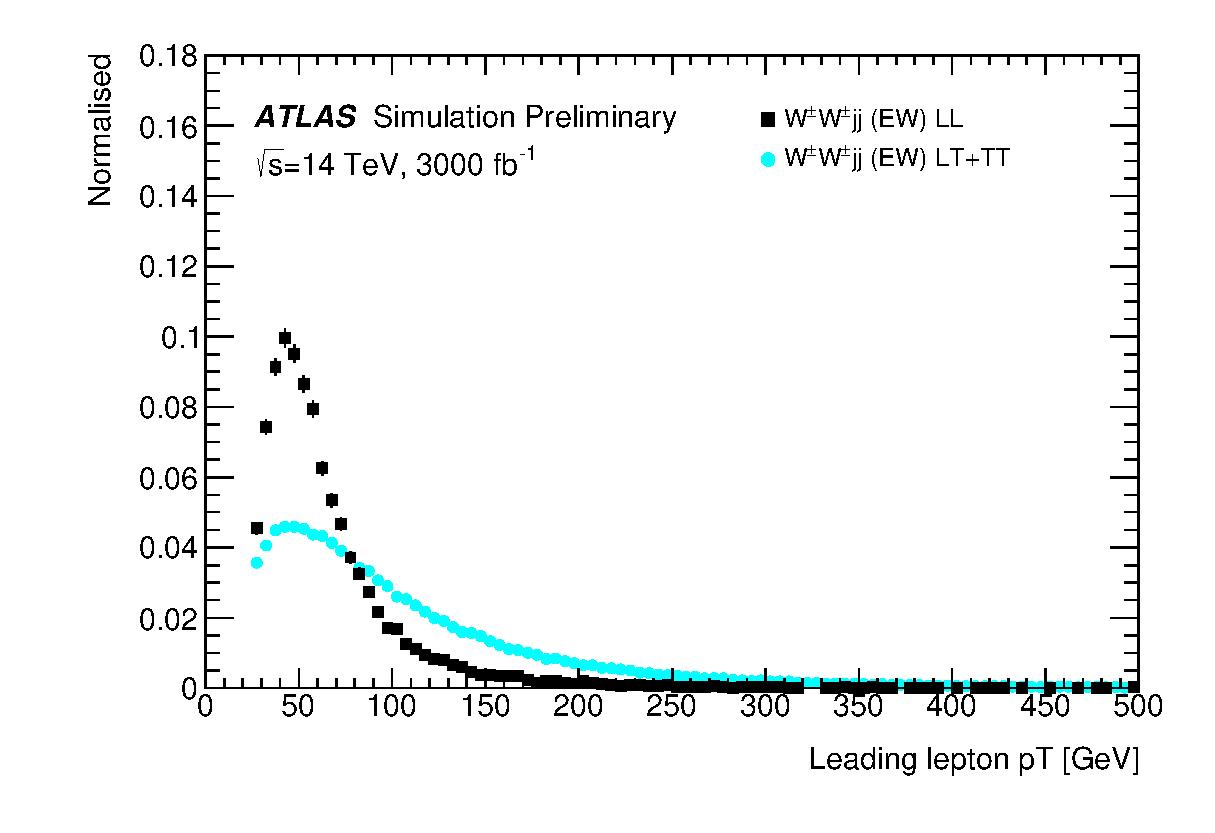
\includegraphics[width=0.8\textwidth]{figs/ssww_upgrade/polarization/lepton0_pt_pass9}\\
  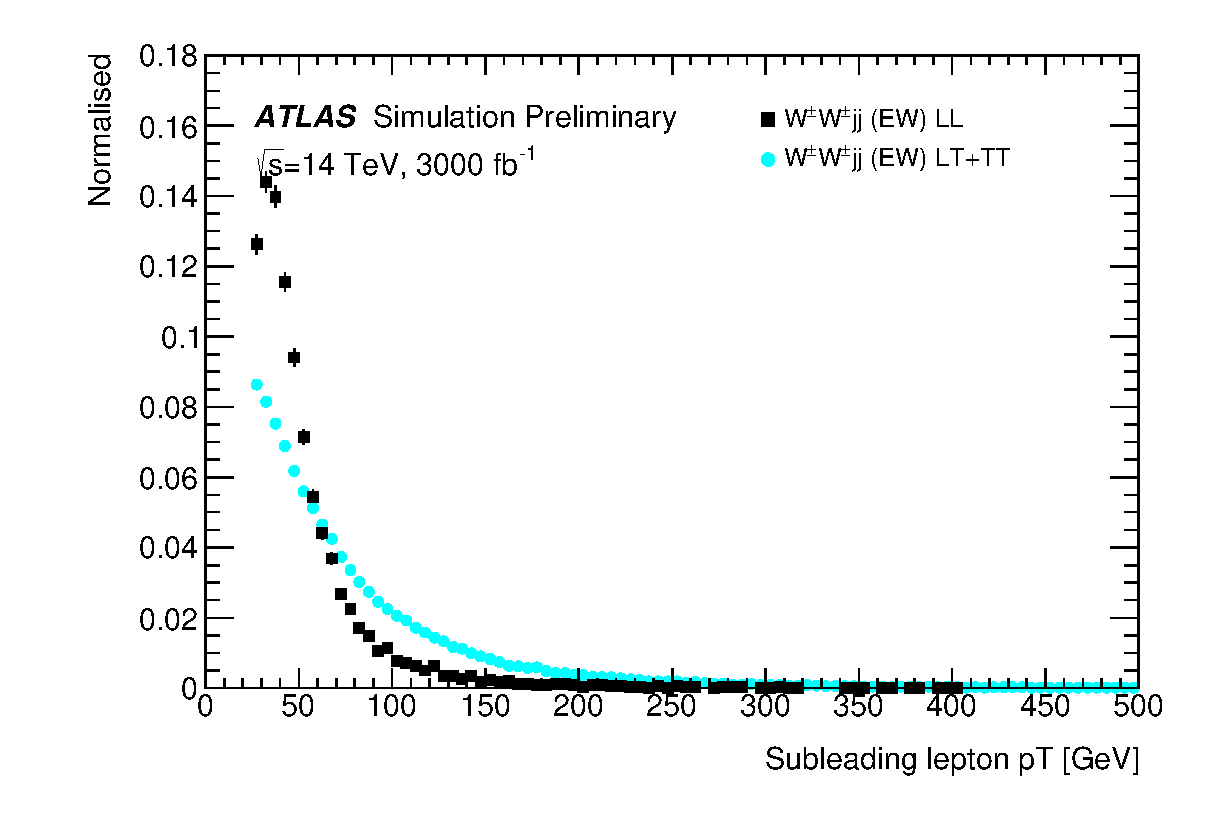
\includegraphics[width=0.8\textwidth]{figs/ssww_upgrade/polarization/lepton1_pt_pass9}
  \caption{Comparison of the leading (top) and subleading (bottom) lepton $\pt$ distributions for purely longitudinal (LL, black) and mixed polarization (LT+TT, cyan) \ssww events.  Plots from \cite{2018.ssww-upgrade-support}.}
  \label{fig:polarization_leppt}
\end{figure}

\begin{figure}[htp]
  \centering
  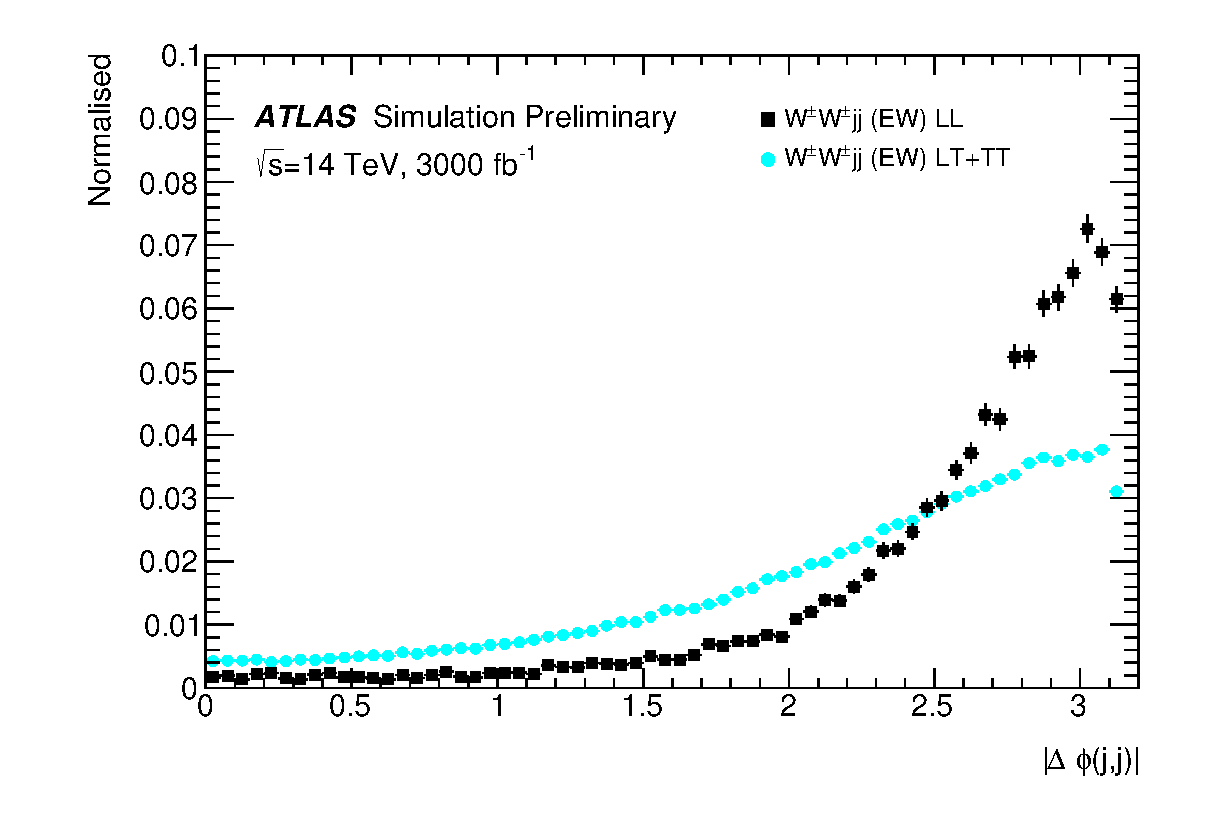
\includegraphics[width=0.8\textwidth]{figs/ssww_upgrade/polarization/dijet_absdphijj_pass9}
  \caption{Comparison of the azimuthal dijet separation ($|\dphijj|$) for purely longitudinal (LL, black) and mixed polarization (LT+TT, cyan) \ssww events.  Plot from \cite{2018.ssww-upgrade-support}.}
  \label{fig:polarization_dphijj}
\end{figure}
